\section{Stable Mechanism on GDN-2}
\label{appendix:stable_gdn2}

\subsection{Problem Formulation}

We consider a general recursive update of the form
\begin{equation}
S_t = P_t S_{t-1} + B_t.
\end{equation}
Define the propagation matrix $\Phi_{t:i} = P_t P_{t-1}\cdots P_i$. Expanding the recursion yields
\begin{equation}
S_t = \Phi_{t:1} S_0 + \sum_{i=1}^{t} \Phi_{t:i+1} B_i.
\end{equation}
Setting $S_0=0$, we obtain
\begin{equation}
S_t = \sum_{i=1}^{t} \Phi_{t:i+1} B_i.
\end{equation}
Assuming $\lVert P_t\rVert \le \rho$ and $\lVert B_t\rVert \le R$, an upper bound of $\lVert S_t\rVert$ is
\begin{equation}
\lVert S_t\rVert \le R\sum_{j=0}^{t-1} \rho^j,
\end{equation}
that is,
\begin{equation}
\lVert S_t\rVert
\le
\begin{cases}
\displaystyle R\frac{1-\rho^t}{1-\rho}, & 0\le \rho<1,\\[0.8em]
\displaystyle tR, & \rho=1,\\[0.6em]
\displaystyle R\frac{\rho^t-1}{\rho-1}, & \rho>1.
\end{cases}
\end{equation}
Therefore, when $\rho<1$, we have
$\lVert S_t\rVert \le \frac{R}{1-\rho}$ as $t\to\infty$, and the update is bounded; we call such a recursion a \emph{stable update}.

Next, we analyze the vector-form GDN-2 update:
\begin{equation}
S_t = \bigl(I - k_t^\top (b_t \odot k_t)\bigr) D_t S_{t-1} + k_t^\top (w_t \odot v_t),
\end{equation}
where $D_t=\mathrm{Diag}(d_t)$ is diagonal, $d_t,b_t,w_t\in(0,1)$, and $\lVert k_t\rVert_2=1,\lVert v_t\rVert_2\leq g$, $g$ is a boundary of $v$'s norm.

This update is not stable in general. Let
$A_t = I - k_t^\top (b_t \odot k_t)$, $P_t=A_t D_t$, and $B_t=k_t^\top (w_t \odot v_t)$.

We omit the time index and define
\begin{equation}
a=b\odot k,\quad \rho = ka^\top,\quad m=\lVert a\rVert_2^2.
\end{equation}
Then
\begin{equation}
\rho=\sum_i b_i k_i^2,\qquad m=\sum_i b_i^2 k_i^2,
\end{equation}
and $\rho\in(0,1)$, $m\in[\rho^2,\rho)$.

Decompose $a$ into the component parallel to $k$ and the orthogonal component. Let $e$ be a unit vector such that $ek^\top = 0$ and $\lVert e\rVert_2=1$. Define $\gamma^2=m-\rho^2$, then
\begin{equation}
a = \rho k + \gamma e.
\end{equation}
Using the basis $\{k,e\}$, we have
\begin{equation}
A = I - k^\top a
= \begin{bmatrix}
1-\rho & -\gamma\\
0 & 1
\end{bmatrix}\oplus I_{K-2}.
\end{equation}
Hence
\begin{equation}
eA^\top = e - \gamma k,\qquad \lVert eA^\top\rVert_2^2 = 1+\gamma^2 \geq 1.
\end{equation}
This shows that along the $e$ direction, whenever $\gamma\neq 0$, the update amplifies energy, and $A$ may lead to an unstable recursion. Moreover,
\begin{equation}
\gamma=0 \iff a \parallel k.
\end{equation}
Thus, if we only consider $A$, a prerequisite for stability is that $b\odot k$ must be colinear with $k$.

We further analyze $A$ by focusing on its $2\times 2$ non-trivial block $A_2$ and considering $A_2^\top A_2$. Its trace is $T=2-2\rho+m$ and its determinant is $\det(A_2^\top A_2)=(1-\rho)^2$. The squared spectral norm (i.e., the largest singular value squared) is
\begin{equation}
\lVert A_2\rVert_2^2 = \lambda_+ = \frac{T+\sqrt{T^2-4(1-\rho)^2}}{2} \ge 1.
\end{equation}
In particular, the spectral norm squared of the full $A_2$ block is
\begin{equation}
\lVert A\rVert_2^2 = \max\{1,\lambda_+\}=\lVert A_2\rVert^2.
\end{equation}
Since $m<\rho$, we have
\begin{equation}
\lambda_+ < \frac{2-\rho+\sqrt{\rho(4-3\rho)}}{2}.
\end{equation}
The right-hand side achieves its maximum $\frac{4}{3}$ at $\rho=\frac{1}{3}$, hence
\begin{equation}
1 \le \lVert A\rVert_2 < \frac{2}{\sqrt{3}}.
\end{equation}
This gives an upper bound on the spectral norm of $A$. When both $A$ and $D$ are considered in the update, if $\lVert D\rVert_2\le \overline{d}$, then
\begin{equation}
\lVert P\rVert_2 = \lVert AD\rVert_2 \le \frac{2}{\sqrt{3}}\,\overline{d}.
\end{equation}
To ensure uniform contraction bound for $P_t$ less than 1, a sufficient condition is $\overline{d} < \frac{\sqrt{3}}{2}\approx 0.866$. Since $P_t S_{t-1}$ does not always amplify, $\overline{d}<0.866$ is a sufficient condition for stability in the worst case.
This condition guaranties uniform contraction of the homogeneous recursion. If the additive inputs $B_t=k_t^\top(w_t\odot v_t)$ are uniformly bounded, then the resulting inhomogeneous recursion is uniformly bounded as well.
Under this condition, the half-life of the forget gate $D$,
\begin{equation}
t_{1/2}=\frac{\ln 2}{-\ln d}=\frac{\ln 2}{-\ln\sqrt{3}/{2}}\approx 4.82,
\end{equation}
is only about 5 tokens.

\subsection{Solution: Symmetrization Fix}

Note that in the GDN-2 update, the $A$ term can be written as
\begin{equation}
A = I - k^\top (b\odot k) = I - k^\top k\,\mathrm{Diag}(b).
\end{equation}
The instability stems from the fact that $A$ is not symmetric. We therefore move $\mathrm{Diag}(b)$ to both $k$ to make $A$ symmetric:
\begin{equation}
A = I - \text{Diag}(\sqrt{b})\,k^\top k\,\text{Diag}(\sqrt{b}).
\end{equation}
Further, we can rewrite it as
\begin{equation}
A = I - (\sqrt{b}\odot k)^\top(\sqrt{b}\odot k).
\end{equation}
With this symmetrization fix, we obtain Stable GDN-2 (SGDN-2), whose update is
\begin{equation}
S_t = \bigl(I-(\sqrt{b_t}\odot k_t)^\top(\sqrt{b_t}\odot k_t)\bigr) D_t S_{t-1}
+ (\sqrt{b_t}\odot k_t)^\top(w_t\odot v_t).
\end{equation}
According to the analysis above, the two vectors in SGDN-2 are naturally colinear (i.e., $\gamma=0$), which avoids the unstable update mechanism.

Geometrically, the symmetrized erase step acts separately
on the component parallel to $u=\sqrt{b}\odot k$ and its
orthogonal complement, with no coupling between these two
orthogonal subspaces. Considering the erase step alone,
with $D=I$ and no write term, the parallel component is
scaled by $1-\lVert u\rVert_2^2$, while the orthogonal
component remains unchanged. Under the stated assumptions,
$0<\lVert u\rVert_2^2<1$; hence, the map contracts along $u$
without expanding any orthogonal direction and is
non-expansive in the Euclidean norm.

In contrast, GDN-2 computes the erase magnitude using
$a=b\odot k$ but applies the correction along $k$.
For the input $y=e$, this gives $y'=e-\gamma k$.
Since $e$ and $k$ are orthogonal, the correction increases
the squared norm from $1$ to $1+\gamma^2$ whenever
$\gamma\neq0$.
Figure~\ref{fig:stable_gdn2_geometry} illustrates the resulting
non-expansive map and contrasts it with a GDN-2 erase step
that increases the norm of the same input $y=e$.

\begin{figure}
    \centering
    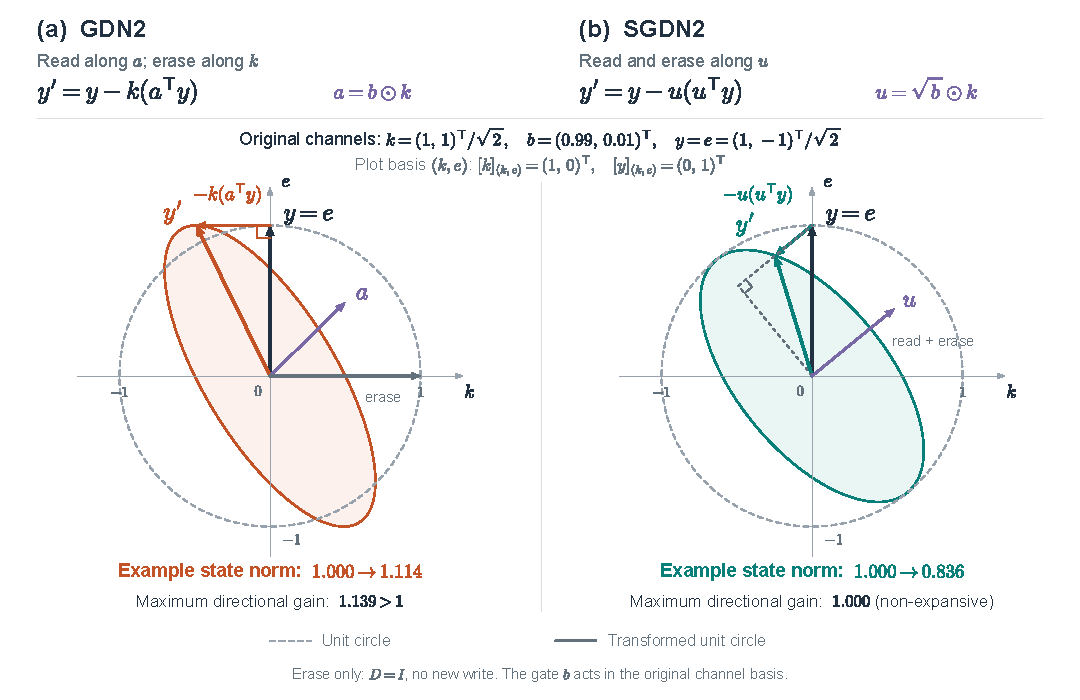
\includegraphics[width=0.8\linewidth]{figures/stable_gdn2_erase_geometry.pdf}
    \caption{An analytical single-step erase example with $D=I$ and no write term.
    Both panels use the same input $y=e$ and orthonormal $\{k,e\}$ basis.}
    \label{fig:stable_gdn2_geometry}
\end{figure}
